\documentclass[a4paper,12pt]{article}

\usepackage{graphicx}

\DeclareGraphicsExtensions{.pdf}

\usepackage{fancyhdr}
\pagestyle{fancy}
\fancyhf{}
\rhead{Dominic Moylett - dm1905@my.bristol.ac.uk}
\cfoot{Page \thepage}

\begin{document}
    \begin{center}
        \section*{Fault Tolerant Computation and VLSI Testing}
        \subsection*{Assignment 1}
    \end{center}

    \begin{enumerate}

        \item Availability = $\frac{120}{120 + 10} = \frac{120}{130} = 0.92$

        \item Fault avoidance is trying to avoid faults occuring altogether.

        Fault tolerance is accepting that faults will happen but trying to ensure that faults do no propogate to errors and failures.

        Fault tolerance is easier to implement than fault avoidance.

        \item
        \begin{itemize}
            \item Ultra-reliable systems are systems which perform critical real-time computation, such as avionic computers for unstable aircraft.
            \item Safety-critical systems are systems where safety is the primary objective, such as nuclear power plants.
            \item Mission-critical systems are systems where a particular mission is primarily important, such as manned spacecraft.
            \item Long-life systems are systems where maintenance or repair are impossible, such as satellites.
            \item Highly-available systems are systems where downtime is expensive, such as cloud computers.
        \end{itemize}

        The advantage of hybrid systems is that many applications require a combination of these properties. For example, a manned spacecraft should be both mission critical and safety critical.

        The disadvantage is that combining these properties is difficult, such as a system which is both ultra-reliable and long-life.

        \item $\lambda_{Sys} = 0.002 * 400 = 0.8$ failures in every 1000 hours.

        $MTTF = \frac{1000}{\lambda_{Sys}} = 1250$ hours

        $R_{Sys}(2000) = e^{-0.8 * 2} = e^{-1.6} = 0.201$

        \item Assuming we have an ideal voter:

        $R_{Sys}(10) = R_aR_bR_c + R_aR_b(1 - R_c) + R_aR_c(1 - R_b) + R_bR_c(1 - R_a)$

        $= e^{(\lambda_a + \lambda_b + \lambda_c)*10} + e^{(\lambda_a + \lambda_b)*10}(1 - e^{\lambda_c*10})$

        $+ e^{(\lambda_a + \lambda_c)*10}(1 - e^{\lambda_b*10}) + e^{(\lambda_b + \lambda_c)*10}(1 - e^{\lambda_a*10})$

        $= e^{6*10^{-5}} + e^{3*10^{-5}}(1 - e^{3*10^{-5}}) + e^{4*10^{-5}}(1 - e^{2*10^{-5}}) + e^{5*10^{-5}}(1 - e^{1*10^{-5}})$

        $ = 0.9999999989$

        \item First, we need the reliability of one pair of modules:

        $R_{Pair} = R_M^2 + 2R_M(1 - R_M)C$

        Now, we consider this as part of the overall system:

        $R_{Sys} = R_{Pair}^2 + 2R_{Pair}(1 - R_{Pair})C$

        $= (R_M^2 + 2R_M(1 - R_M)C)^2$

        $+ 2(R_M^2 + 2R_M(1 - R_M)C)(1 - R_M^2 - 2R_M(1 - R_M)C)C$

        When plotted on a graph, this looks like the following:

        \begin{center}
            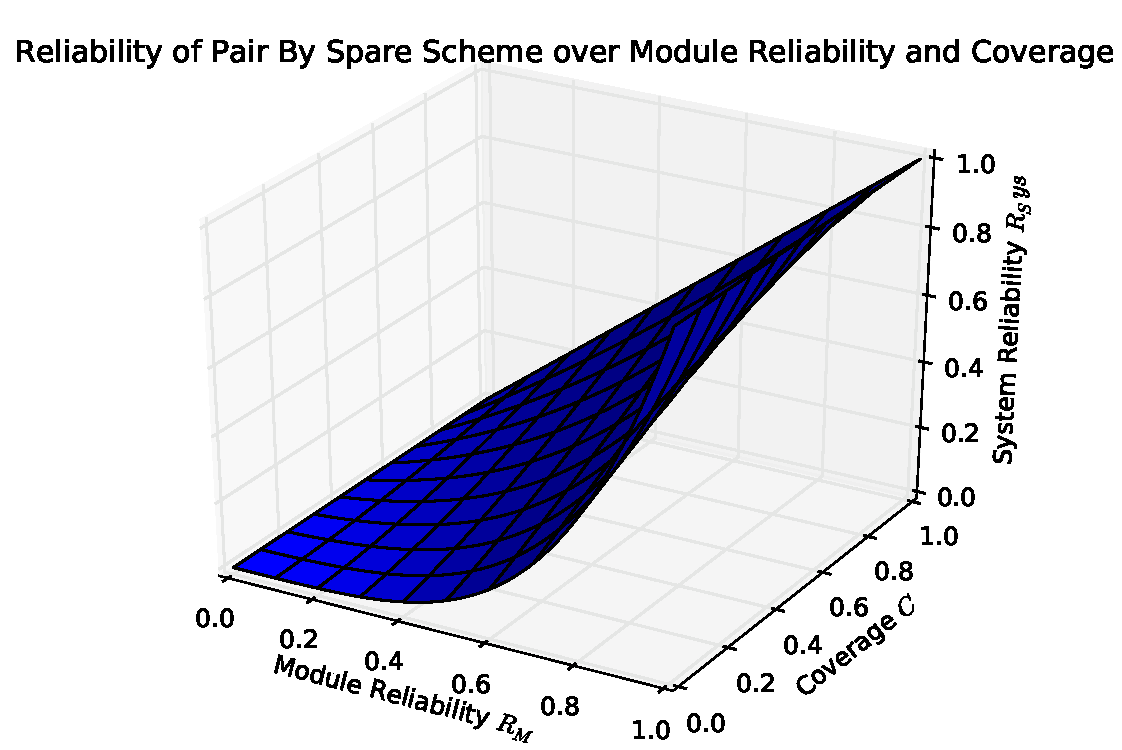
\includegraphics[scale=0.7]{question_6_graph}
        \end{center}

        \item When a module fails in our hybrid system, there are two possibilities:

        \begin{itemize}
            \item If $M_1$ or $M_2$ fail, then we remove that module and are left with two modules.
            \item If $M_3$ fails, then we swap out the module and have a traditional TMR.
        \end{itemize}

        Our system can therefore be modelled by the following equation, assuming that our voter and reconfiguration circuitry are perfect:

        $R_{Sys} = R_M^3 + 2(1 - R_M)R_M^2 + (1 - R_M)(R_M^3 + 3(1 - R_M)R_M^2)$

        By setting $R_M(t) = e^{-0.001t}$, we can see what the reliability of the system looks like compared to standard TMR with no spares. Plotted below is the reliability of both schemes over 4000 hours:

        \begin{center}
            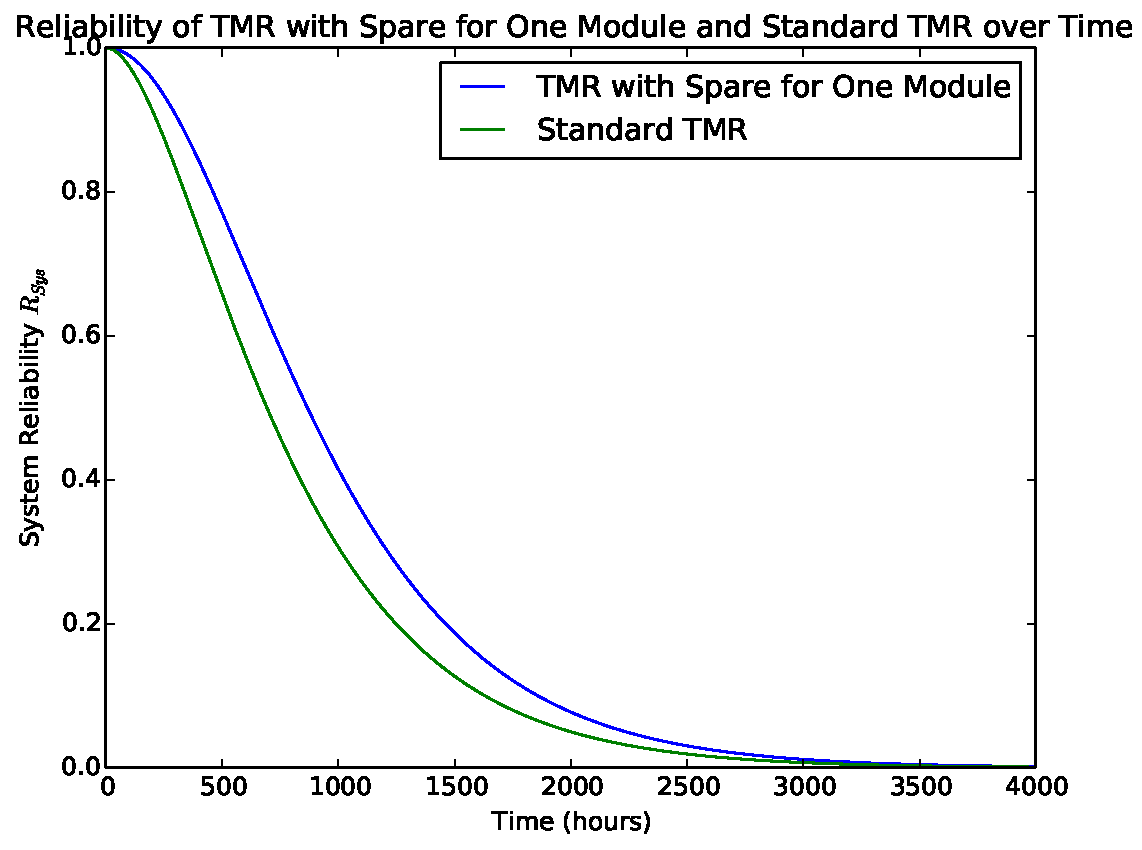
\includegraphics[scale=0.7]{question_7_graph}
        \end{center}

    \end{enumerate}

\end{document}